% To je predloga za poročila o domačih nalogah pri predmetih, katerih
% nosilec je Tomaž Curk. Avtor predloge je Blaž Zupan.
%
% Seveda lahko tudi dodaš kakšen nov, zanimiv in uporaben element, 
% ki ga v tej predlogi (še) ni. Več o LaTeX-u izveš na
% spletu, na primer na http://tobi.oetiker.ch/lshort/lshort.pdf.
%
% To predlogo lahko spremeniš v PDF dokument s pomočjo programa
% pdflatex, ki je del standardne instalacije LaTeX programov.

\documentclass[a4paper,11pt]{article}
\usepackage{a4wide}
\usepackage{fullpage}
\usepackage[utf8x]{inputenc}
\usepackage[slovene]{babel}
\selectlanguage{slovene}
\usepackage[toc,page]{appendix}
\usepackage[pdftex]{graphicx} % za slike
\usepackage{setspace}
\usepackage{color}
\definecolor{light-gray}{gray}{0.95}
\usepackage{listings} % za vključevanje kode
\usepackage{hyperref}
\renewcommand{\baselinestretch}{1.2} % za boljšo berljivost večji razmak
\renewcommand{\appendixpagename}{Priloge}

\lstset{ % nastavitve za izpis kode, sem lahko tudi kaj dodaš/spremeniš
	language=Python,
	basicstyle=\footnotesize,
	basicstyle=\ttfamily\footnotesize\setstretch{1},
	backgroundcolor=\color{light-gray},
}

\title{Domača naloga 2}
\author{Jernej Habjan (63150106)}
\date{\today}

\begin{document}
	
	\maketitle
	\renewcommand\thesubsection{\Alph{subsection}}

	
	\section{Uvod}
	
	Naloga je poiskati osamelce, ugotoviti njihove lastnosti in na kakšen način odstopajo od večine. Ugotoviti je potrebno tudi kakšni porazdelitvi se podatki prilegajo. Drugi del naloge je iskanje sorodnih primerov v podatkih ali grupiranje.
	
	\section{Iskanje osamelcev}

	\subsection{Naključna spremenljivka}
		Za naključno spremenljivko sem izbral "ratings", ki govori o ocenah filmov. Za iskanje osamelcev bom gledal njeno varianco. Tisti filmi, pri katerih imajo ocene največjo varianco pomeni, da so si gledalci najbolj neenotni.

		
	\subsection{Porazdelitev naključnostne spremenljivke}
	
		Na spodnji sliki prikazujem histogram variance ocen filmov. Pri grafu sem upošteval vse filme, tudi tiste z manj ocenami, kjer so si gledalci še posebej neenotni.
		Pri filmih s skoraj nič ocenami so si gledalci lahko zelo neenotni, ali pa vsi ocenijo isto oceno, čeprav to ni pričakovana ocena.\\


		Slika 1 - iz neznanih razlogov mi ne pokaže slike v tem razdelku ampak malo nižje - Glej Slika 1

		\begin{figure}[!htb]
			\begin{center}
				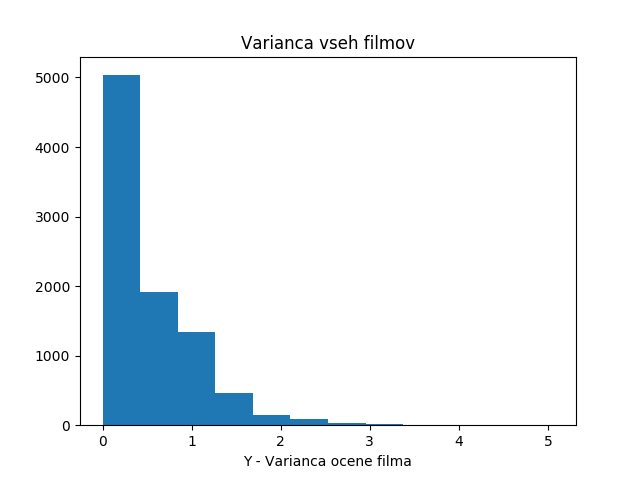
\includegraphics[scale=1.0]{slike/graph1_varianca.png}
				\caption{Graf prikazuje porazdelitev variance ocen}
				\label{slika1}
			\end{center}
		\end{figure}

	
	\subsection{Znana porazdelitev}
		Spremenjivka spominja na Beta porazdelitev. Za večino filmov se ocenjevalci strinjajo o njegovi oceni, tako da so si dovolj skladni in je varianca blizu 0. Ni pa čisto 0, saj da se ljudje čisto strinjajo mora biti a) zelo dober film, b) zelo malo ocenjen film
		
		Krivulja je na začetku zelo strma, doseže svoj vrh in pada. Pri oceni 3 je pa že skoraj vodoravna.
		
		\begin{figure}[!htb]
			\begin{center}
				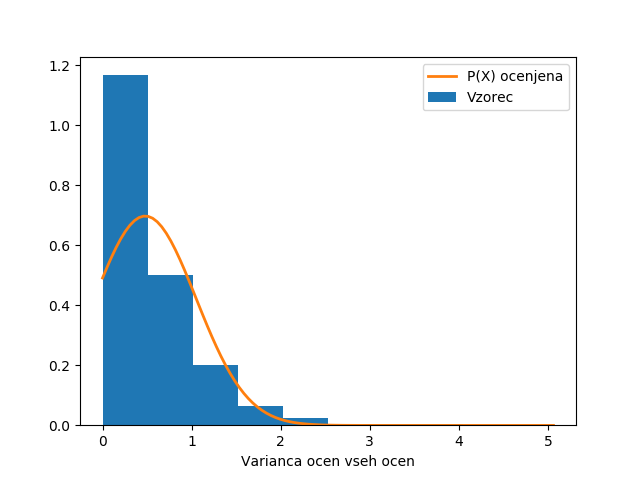
\includegraphics[scale=1.0]{slike/graph2_porazdelitve.png}
				\caption{Graf Beta porazdelitve in njene pričakovane ocene prikazano z oranžno črto}
				\label{slika2}
			\end{center}
		\end{figure}

		Porazdelitev bi lahko spominjala tudi na Gamo porazdelitev, saj pada, vendar se ji beta bolj prilega.
	\subsection{Ocenitev parametrov}
		Porazdelitev sem narisal s pomočjo normalne porazdelitve kjer je bilo potrebno izračunati mi in varianco.
		\begin{lstlisting}

Vse ocene:     mi = 0.4789 in varianca = 0.3268
	
		\end{lstlisting}
		
		Poskusil sem prilegati funkcijo z beta "beta.fit(sample)" vendar je po Y maksimalna vrednost 5000 in bi morala biti funkcija beta zelo strma in se neuspešno prilega.\\\\
		Glej sliko 3 na koncu dokumenta.
		
	
		

	\subsection{Najbolj prilegajoča porazdelitev}
		Rekel bi, da se porazdelitev najbolj prilagaja Beta porazdelitvi vendar izračunana z normalno porazdelitvijo s parametroma mi = 0.4789 in varianca = 0.3268

		
	\subsection{Filmi z p 5 procentov}
		Lista filmov je priložena v posebni datoteki "top5PercVariance.txt" ki je podana med prilogami zraven datoteke
	
	
	\section{Gručenje filmov}

	\subsection{Algoritem in mere podobnosti}
		Izbral sem algoritem hierarhičnega gručenja silhuetni score. Metoda KNN ne učinkuje dobro, saj hitro izračuna rezultat, vendar vrne rezultat v obliki stotih atributov, ki jih pa nemorem predstaviti.
		Algoritem silhuetni score je pa počasnejši, saj mora preračunati veliko podmatrik, ampak je dovolj hiter za 100 filmov.\\
		Pri temu algoritmu sem uporabil za metodo povezovanja - complete in za mero razdalje euclidean. Tadva parametra sem izbral tako, da sem testiral njihovo maksimalno oceno "adjusted mutual info score"
		
		Potek algoritma:\\
		Prvo sem izbral 100 najbolj gledanih filmov, ocenjevalce in njihove ocene.\\
		Potem sem naredil matriko, ki ima atribute movieId in ocenjevalce in ima 100 zapisov.\\
		Če uporabnik ni ocenil, filma, sem na tisto mesto napisal povprečje ocen tega ocenjevalca in ocen filma. Pred tem sem napisal notri oceno 0 in je prišlo do zelo slabših rezultatov.
		Potem sem iz te matrike ugotovil najboljše atribute za silhuetni score - t, metodo, mero.\\
		Nakoncu sem še narisal dendrogram z najboljšimi pridobljenimi atributi - glej Slika 3
				
	\subsection{Skupine}
		Prav tako sem z algoritmom ki je izračunal maksimalno "adjusted mutual info score" izračunal tudi parameter t, ki pove kje porezati drevo.
		T je znašal 16 in na tej stopnji bi nastalo 9 skupin.
		

	\subsection{Vizualizacija}
		
	\begin{figure}[!htb]
		\begin{center}
			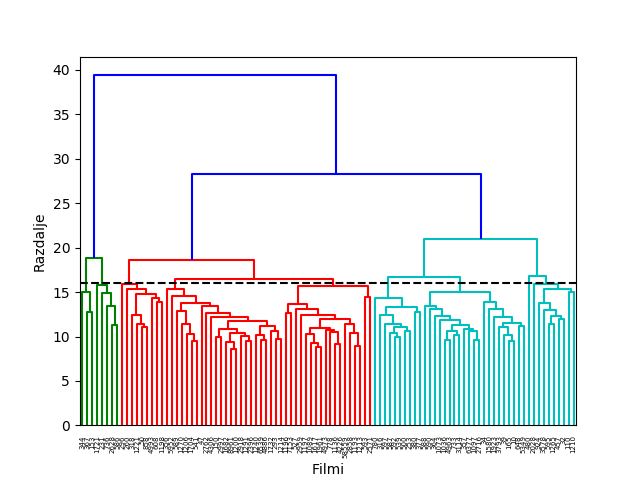
\includegraphics[scale=1.0]{slike/graph4_dendrogram.png}
			\caption{Dendogram s parametrom t = 16, metodo complete in mero euclidean}
			\label{slika4}
		\end{center}
	\end{figure}

	
	\subsection{Rezultati}
		Adjusted mutual info score je znašal 0.32 pri T = 16, metoda = "complete", mera = "euclidean"
		Najbolši rezultat je znašal 0.36, vendar metoda "single" vizualno ni grafa razbil na tako lepe dele kot jih complete, zato sem izbral drugo najboljšo kombinacijo.
		Vizualno graf zgleda lepo razdelan in ima med nekaterimi skupinami veliko razdaljo, kar jih dobro ločuje. \\
		Prav tako sem poskusil z KNN vendar ne vem kako dobre rezultate sem dobil, saj je atributov toliko, kolikor je uporabikov in  jih ne morem prikazati na 2d ravnini.
		
		Da filme razbijemo na 9 skupin se mi zdi smiselno, tako da ni prišlo do prevelikega prileganja, kot tudi ni premalo skupin, saj je le 19 žanrov in že žanri sami zagotovo razdelijo uporabnike in filme na skupine.


	\section{Izjava o izdelavi domače naloge}
	Domačo nalogo in pripadajoče programe sem izdelal sam.
	
	\appendix
	\appendixpage
	\section{\label{app-res}Slike}
	Slike sem priložil v mapo slike.		
	
		
	\section{\label{app-code}Programska koda}
	Programsko kodo sem zapakiral v datoteko koda.zip in jo priložil k poročilu.
	Prav tako sem v ta zip priložil datoteke potrebne za zagon programa.
	Za zagon programa odprite main.py datoteko in v funckciji main odkomentirajte funkcijo ki jo hočete testirati.


\begin{figure}[!htb]
	\begin{center}
		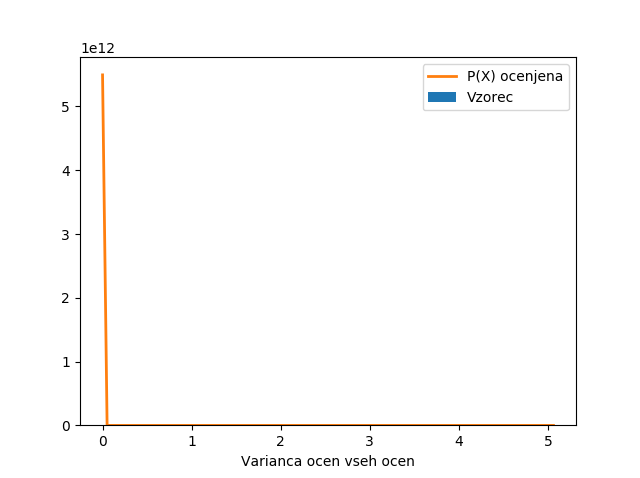
\includegraphics[scale=1.0]{slike/graph3_fit.png}
		\caption{Neuspešen poskus prileganja z beta.fit(sample)}
		\label{slika3}
	\end{center}
\end{figure}


	
\end{document}
